\chapter{Background}
\label{ch:background}

This chapter provides the necessary theoretical background for understanding the proposed method. We begin with the fundamentals of \gls{ct} imaging, followed by a detailed explanation of truncation artifacts and their causes. We then introduce the mathematical foundations of diffusion models and the Cold Diffusion framework.

\section{Computed Tomography Fundamentals}

\subsection{X-ray Attenuation and the Radon Transform}

\gls{ct} imaging is based on the principle of X-ray attenuation. When an X-ray beam passes through matter, its intensity decreases exponentially according to the Beer-Lambert law:
%
\begin{equation}
I = I_0 \exp\left(-\int_L \mu(\mathbf{x}) \, \mathrm{d}s\right)
\end{equation}
%
where $I_0$ is the incident intensity, $I$ is the transmitted intensity, $\mu(\mathbf{x})$ is the linear attenuation coefficient at position $\mathbf{x}$, and $L$ is the X-ray path through the object.

The negative logarithm of the intensity ratio gives the \textit{line integral}:
%
\begin{equation}
p = -\ln\left(\frac{I}{I_0}\right) = \int_L \mu(\mathbf{x}) \, \mathrm{d}s
\label{eq:line_integral}
\end{equation}

A collection of such line integrals for different X-ray paths forms the \textit{projection data} or \textit{sinogram}. Mathematically, this is described by the \textit{Radon transform}~\cite{kak2001principles}:
%
\begin{equation}
\mathcal{R}\{\mu\}(\theta, t) = \int_{-\infty}^{\infty} \mu(t\cos\theta - s\sin\theta, t\sin\theta + s\cos\theta) \, \mathrm{d}s
\label{eq:radon_transform}
\end{equation}
%
where $\theta$ is the projection angle and $t$ is the detector position perpendicular to the ray direction.

\subsection{Sinogram Representation}

In practice, \gls{ct} scanners acquire projections at discrete angles $\theta_i \in [0, 2\pi)$ and detector positions $t_j$. The resulting 2D array $\mathbf{P} \in \mathbb{R}^{N_\theta \times N_t}$ is called the \textit{sinogram}, where $N_\theta$ represents the number of projection angles (typically 360-1000), $N_t$ denotes the number of detector elements (typically 512-1024), and $\mathbf{P}_{ij}$ contains the projection value at angle $\theta_i$ and detector position $t_j$.

The sinogram formation process follows the standard Radon geometry: a point in the object domain traces a sinusoidal curve in the sinogram domain, which motivates the term \textit{sinogram}.

\subsection{Image Reconstruction: Filtered Backprojection}

The goal of \gls{ct} reconstruction is to recover the attenuation map $\mu(\mathbf{x})$ from the sinogram $\mathbf{P}$. The most widely used method is \gls{fbp}~\cite{kak2001principles}, which consists of two steps:

\paragraph{1. Filtering} Apply a ramp filter (or windowed ramp filter) to each projection:
%
\begin{equation}
\tilde{p}(\theta, t) = p(\theta, t) \ast h_{\text{ramp}}(t)
\end{equation}
%
where $\ast$ denotes convolution and $h_{\text{ramp}}$ is the ramp filter kernel in spatial domain, or equivalently in Fourier domain:
%
\begin{equation}
\tilde{P}(\theta, \omega) = P(\theta, \omega) \cdot |\omega|
\end{equation}

\paragraph{2. Backprojection} Sum filtered projections over all angles:
%
\begin{equation}
\hat{\mu}(x, y) = \int_0^{\pi} \tilde{p}(\theta, x\cos\theta + y\sin\theta) \, \mathrm{d}\theta
\end{equation}

In discrete form:
%
\begin{equation}
\hat{\mu}_{mn} = \sum_{i=1}^{N_\theta} \tilde{p}(\theta_i, x_m\cos\theta_i + y_n\sin\theta_i)
\label{eq:fbp_discrete}
\end{equation}

\gls{fbp} is computationally efficient and provides exact reconstruction under ideal conditions (complete angular coverage, sufficient angular sampling, infinite detector width). However, it is highly sensitive to data incompleteness, including truncation.

For cone-beam CT, the \gls{fdk} algorithm extends \gls{fbp} with a weighted backprojection scheme to handle divergent beams~\cite{feldkamp1984practical}. In this work, cone-beam projection and reconstruction operators are implemented using PyRoNN~\cite{syben2019pyronn}, which provides GPU-accelerated forward and backprojection routines aligned with the \gls{fdk}-style geometry.

\section{Truncation Artifacts in CT}

\subsection{Definition and Causes}

\textit{Truncation artifacts} occur when parts of the patient's anatomy extend beyond the scanner's \gls{fov}, resulting in incomplete projection data~\cite{ohnesorge2000efficient, hsieh2015computed}. This violates a fundamental assumption of \gls{fbp}: that all projection rays pass entirely through the object and that attenuation outside the \gls{fov} is zero.

Formally, let $\Omega$ denote the region inside the \gls{fov} and $\bar{\Omega}$ the region outside. The \gls{ct} scanner measures:
%
\begin{equation}
p_{\text{measured}}(\theta, t) = \int_{L \cap \Omega} \mu(\mathbf{x}) \, \mathrm{d}s
\end{equation}
%
while the complete projection would be:
%
\begin{equation}
p_{\text{complete}}(\theta, t) = \int_{L \cap (\Omega \cup \bar{\Omega})} \mu(\mathbf{x}) \, \mathrm{d}s = p_{\text{measured}}(\theta, t) + \underbrace{\int_{L \cap \bar{\Omega}} \mu(\mathbf{x}) \, \mathrm{d}s}_{\text{missing data}}
\end{equation}

The missing contribution from $\bar{\Omega}$ leads to incorrect filtered projections and subsequently to artifacts in the reconstructed image.

\subsection{Types of Truncation}

Truncation can be bilateral (symmetric) when both sides of the object extend beyond the detector, or unilateral/partial when only one side or a subset of angles is affected. This thesis focuses on bilateral truncation as the controlled setting for systematic evaluation.

\subsection{Artifact Manifestations}

Truncation artifacts manifest in the reconstructed image in several ways~\cite{hsieh2015computed}:

\begin{enumerate}
    \item \textbf{Cupping artifacts}: The reconstructed HU values gradually decrease from the \gls{fov} center toward the edges
    \item \textbf{Streak artifacts}: Bright streaks radiate from the truncation boundary
    \item \textbf{Intensity bias}: Overall HU values are systematically underestimated
    \item \textbf{Edge shading}: Dark bands appear near the \gls{fov} boundary
\end{enumerate}

These artifacts can substantially degrade diagnostic quality, especially in quantitative applications such as radiotherapy planning, where accurate HU values are critical.

Figure~\ref{fig:background_truncation_artifacts} illustrates the effect of bilateral truncation on both the sinogram and the reconstructed image.

\begin{figure}[htbp]
\centering
\resizebox{\textwidth}{!}{%
\begin{tikzpicture}[font=\scriptsize]

% ===================== Row 1: complete-data chain =====================
\begin{scope}[shift={(0,0)}]
  \draw[fill=gray!20] (0,0) rectangle (3.2,2.4);
  \foreach \k in {0.3,0.6,0.9,1.2,1.5,1.8,2.1}{
    \draw[gray!70, thick, smooth, domain=0:3.2, samples=60]
      plot (\x, {\k + 0.18*sin(deg(2*\x+\k*1.5))});
  }
  \node[above] at (1.6,2.4) {\textbf{Complete sinogram}};
  \node[below] at (1.6,0)   {$N_t$ detector columns};
  \draw[<->,thin] (0,-0.42) -- (3.2,-0.42) node[midway,below]{full width};
\end{scope}

\begin{scope}[shift={(5.2,0)}]
  \draw[fill=gray!15] (0,0) rectangle (3.2,2.4);
  \draw[fill=gray!35,opacity=0.7] (1.6,1.2) circle (0.85);
  \node[above] at (1.6,2.4) {\textbf{Complete FBP}};
  \node[below] at (1.6,0)   {uniform HU values};
\end{scope}

\draw[->,very thick,>=stealth] (3.4,1.2) -- (5.0,1.2);
\node[above,font=\tiny] at (4.2,1.2) {FBP};
\node[font=\small\bfseries,anchor=east] at (-0.25,1.2) {Complete chain};

% ===================== Row 2: truncated-data chain =====================
\begin{scope}[shift={(0,-4.4)}]
  \draw[fill=gray!20] (0.6,0) rectangle (2.6,2.4);
  \fill[pattern=north east lines, pattern color=red!40] (0,0) rectangle (0.6,2.4);
  \fill[pattern=north east lines, pattern color=red!40] (2.6,0) rectangle (3.2,2.4);
  \draw (0,0) rectangle (3.2,2.4);
  \foreach \k in {0.3,0.6,0.9,1.2,1.5,1.8,2.1}{
    \draw[gray!70, thick, smooth, domain=0.6:2.6, samples=40]
      plot (\x, {\k + 0.18*sin(deg(2*\x+\k*1.5))});
  }
  \node[above] at (1.6,2.4) {\textbf{Truncated sinogram}};
  \node[red!70,font=\tiny] at (0.3,1.2) {missing};
  \node[red!70,font=\tiny] at (2.9,1.2) {missing};
  \draw[<->,thin] (0.6,-0.42) -- (2.6,-0.42) node[midway,below]{$k_c$ cols kept};
\end{scope}

\begin{scope}[shift={(5.2,-4.4)}]
  \draw[fill=gray!15] (0,0) rectangle (3.2,2.4);
  \draw[fill=gray!40,opacity=0.85] (1.6,1.2) circle (0.85);
  \draw[fill=gray!22,opacity=0.9] (1.6,1.2) circle (0.42);
  \draw[red!65, line width=1.1pt, opacity=0.8] (0.0,0.3) -- (3.2,2.1);
  \draw[red!65, line width=1.1pt, opacity=0.8] (0.0,2.1) -- (3.2,0.3);
  \draw[red!65, line width=0.8pt, opacity=0.7] (0.2,0.8) -- (3.0,1.7);
  \draw[red!65, line width=0.8pt, opacity=0.7] (0.2,1.7) -- (3.0,0.8);
  \node[above] at (1.6,2.4) {\textbf{Truncation artifacts}};
  \node[below, red!70] at (1.6,0) {cupping (center bias) + streaks};
  \draw[->,red!70,thin] (3.35,2.20) -- (2.25,1.80);
  \node[red!70,font=\tiny,anchor=west,fill=white,inner sep=1pt] at (3.38,2.22) {streaks};
  \draw[->,red!70,thin] (3.35,0.40) -- (2.00,0.95);
  \node[red!70,font=\tiny,anchor=west,fill=white,inner sep=1pt] at (3.38,0.38) {cupping};
\end{scope}

\draw[->,very thick,>=stealth,red!70] (3.4,-3.2) -- (5.0,-3.2);
\node[above,font=\tiny,red!70] at (4.2,-3.2) {FBP};
\node[font=\small\bfseries,anchor=east,red!70] at (-0.25,-3.2) {Truncated chain};

% ---- relation between rows (routed along the left side to avoid all content) ----
\draw[->,very thick,>=stealth,rounded corners=4pt]
  (0,0.3) -- (-0.8,0.3) -- (-0.8,-2.3) -- (0,-2.3);
\node[left,font=\tiny] at (-0.8,-1.0) {truncate};

\end{tikzpicture}
}
\caption{Illustration of the truncation effect in sinogram and image domains. Left pair: a complete sinogram (all detector columns present) and its corresponding artefact-free FBP reconstruction. Right pair: the same sinogram with bilateral truncation (hatched regions are missing) and the resulting FBP reconstruction, which exhibits characteristic cupping and streak artefacts caused by the missing projection data.}
\label{fig:background_truncation_artifacts}
\end{figure}

\section{Diffusion Models}

\subsection{Denoising Diffusion Probabilistic Models (DDPM)}

\gls{ddpm}~\cite{ho2020denoising} is a class of generative models that learns to reverse a gradual noising process. In this thesis, the DDPM baseline is used in a \emph{conditional} restoration setting, where the condition is built from the truncated sinogram and its truncation mask. The model still follows the standard Gaussian-noise forward process and denoising objective:

\paragraph{Forward Process (Noising)} Starting from data $\mathbf{x}_0 \sim q(\mathbf{x}_0)$, progressively add Gaussian noise over $T$ steps:
%
\begin{equation}
q(\mathbf{x}_t \mid \mathbf{x}_{t-1}) = \mathcal{N}(\mathbf{x}_t; \sqrt{1-\beta_t}\mathbf{x}_{t-1}, \beta_t \mathbf{I})
\end{equation}
%
where $\{\beta_t\}_{t=1}^T$ is a variance schedule (typically increasing). Using the reparameterization trick, this can be written in closed form:
%
\begin{equation}
\mathbf{x}_t = \sqrt{\bar{\alpha}_t}\mathbf{x}_0 + \sqrt{1-\bar{\alpha}_t}\boldsymbol{\epsilon}, \quad \boldsymbol{\epsilon} \sim \mathcal{N}(\mathbf{0}, \mathbf{I})
\end{equation}
%
where $\alpha_t = 1 - \beta_t$ and $\bar{\alpha}_t = \prod_{s=1}^t \alpha_s$.

\paragraph{Reverse Process (Denoising)} Learn a neural network $\boldsymbol{\epsilon}_\theta$ to predict the noise and reverse the process:
%
\begin{equation}
p_\theta(\mathbf{x}_{t-1} \mid \mathbf{x}_t, \mathbf{c}) = \mathcal{N}(\mathbf{x}_{t-1}; \boldsymbol{\mu}_\theta(\mathbf{x}_t, t, \mathbf{c}), \tilde{\beta}_t \mathbf{I})
\end{equation}
%
where the predicted mean can be computed as:
%
\begin{equation}
\boldsymbol{\mu}_\theta(\mathbf{x}_t, t, \mathbf{c}) = \frac{1}{\sqrt{\alpha_t}}\left(\mathbf{x}_t - \frac{\beta_t}{\sqrt{1-\bar{\alpha}_t}}\boldsymbol{\epsilon}_\theta(\mathbf{x}_t, t, \mathbf{c})\right)
\end{equation}

\paragraph{Training Objective} The model is trained to predict the noise $\boldsymbol{\epsilon}$:
%
\begin{equation}
\mathcal{L}_{\text{simple}} = \mathbb{E}_{t, \mathbf{x}_0, \boldsymbol{\epsilon}}\left[\|\boldsymbol{\epsilon} - \boldsymbol{\epsilon}_\theta(\mathbf{x}_t, t, \mathbf{c})\|^2\right]
\label{eq:ddpm_loss}
\end{equation}

\paragraph{Condition Definition} For the truncation-correction baseline, the condition is written as $\mathbf{c} = [\mathbf{x}_{\text{trunc}}, \mathbf{M}]$, where $\mathbf{x}_{\text{trunc}}$ is the truncated sinogram and $\mathbf{M}$ is the binary visibility mask.

\paragraph{Sampling} During restoration, sampling starts from noise $\mathbf{x}_T \sim \mathcal{N}(\mathbf{0}, \mathbf{I})$ and iteratively denoises while keeping $\mathbf{c}$ fixed:
%
\begin{equation}
\mathbf{x}_{t-1} = \frac{1}{\sqrt{\alpha_t}}\left(\mathbf{x}_t - \frac{1-\alpha_t}{\sqrt{1-\bar{\alpha}_t}}\boldsymbol{\epsilon}_\theta(\mathbf{x}_t, t, \mathbf{c})\right) + \sigma_t \mathbf{z}, \quad \mathbf{z} \sim \mathcal{N}(\mathbf{0}, \mathbf{I})
\end{equation}

\subsection{Cold Diffusion: Generalization to Arbitrary Degradations}

While \gls{ddpm} uses Gaussian noise as the degradation operator, \textit{Cold Diffusion}~\cite{bansal2022cold} generalizes this to arbitrary deterministic transformations. The key insight is that the iterative refinement mechanism of diffusion models does not inherently require randomness.

\paragraph{Forward Process} Replace Gaussian noise with a deterministic degradation operator $\mathcal{D}$:
%
\begin{equation}
\mathbf{x}_t = \mathcal{D}_t(\mathbf{x}_0)
\end{equation}
%
where $\mathcal{D}_t$ applies increasing levels of degradation. Examples of deterministic degradations include image blurring through convolution with Gaussian kernels of increasing width ($\mathcal{D}_t(\mathbf{x}) = \mathbf{x} \ast g_{\sigma_t}$ with increasing $\sigma_t$), image masking via element-wise multiplication with progressively restrictive masks ($\mathcal{D}_t(\mathbf{x}) = \mathbf{x} \odot \mathbf{M}_t$), or JPEG compression with decreasing quality factors ($\mathcal{D}_t(\mathbf{x}) = \text{JPEG}(\mathbf{x}, q_t)$ with decreasing $q_t$).

\paragraph{Reverse Process} Train a network $f_\theta(\mathbf{x}_t, t)$ to predict the clean image $\mathbf{x}_0$:
%
\begin{equation}
\hat{\mathbf{x}}_0 = f_\theta(\mathbf{x}_t, t)
\end{equation}

Then reconstruct $\mathbf{x}_{t-1}$ by applying a reduced degradation to the prediction:
%
\begin{equation}
\mathbf{x}_{t-1} = \mathcal{D}_{t-1}(\hat{\mathbf{x}}_0)
\label{eq:cold_diffusion_reverse}
\end{equation}

\paragraph{Training Objective} Directly predict $\mathbf{x}_0$:
%
\begin{equation}
\mathcal{L} = \mathbb{E}_{t, \mathbf{x}_0}\left[\|\mathbf{x}_0 - f_\theta(\mathcal{D}_t(\mathbf{x}_0), t)\|^2\right]
\label{eq:cold_diffusion_loss}
\end{equation}
This equation summarizes the standard Cold Diffusion objective in its common $L_2$ form. In the implemented training pipeline of this thesis, we use an $L_1$ objective (see Equation~\ref{eq:training_loss}) to improve reconstruction sharpness and boundary fidelity.
Figure~\ref{fig:background_ddpm_vs_cold_forward} gives an intuitive comparison between the DDPM and Cold Diffusion forward processes.

\begin{figure}[htbp]
\centering
\resizebox{\textwidth}{!}{%
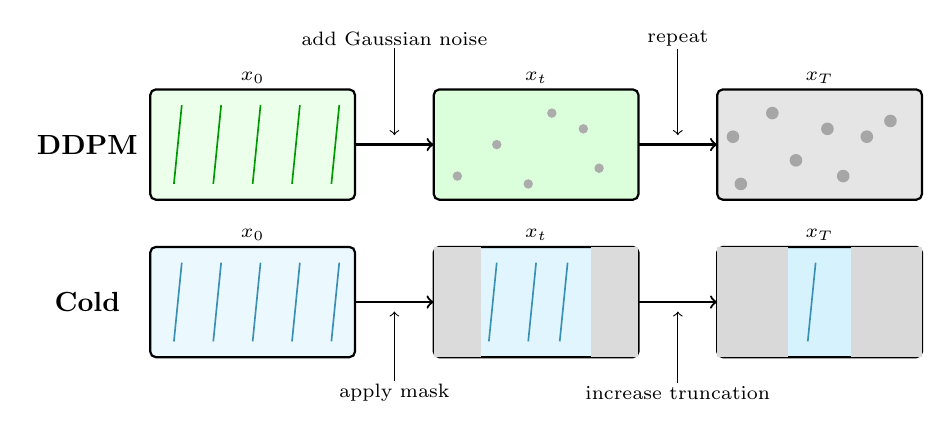
\begin{tikzpicture}[x=1cm,y=1cm,font=\scriptsize]
\node[font=\bfseries] at (-0.8,2.8) {DDPM};
\node[font=\bfseries] at (-0.8,0.8) {Cold};

\draw[thick, rounded corners=2pt, fill=green!8] (0,2.1) rectangle (2.6,3.5);
\node at (1.3,3.65) {\(x_0\)};
\draw[thick, rounded corners=2pt, fill=green!14] (3.6,2.1) rectangle (6.2,3.5);
\node at (4.9,3.65) {\(x_t\)};
\draw[thick, rounded corners=2pt, fill=gray!20] (7.2,2.1) rectangle (9.8,3.5);
\node at (8.5,3.65) {\(x_T\)};
\foreach \x in {0.3,0.8,1.3,1.8,2.3} {\draw[green!60!black, line width=0.6pt] (\x,2.3) -- (\x+0.1,3.3);}
\foreach \x/\y in {3.9/2.4,4.4/2.8,5.1/3.2,5.7/2.5,4.8/2.3,5.5/3.0} {\fill[gray!65] (\x,\y) circle (0.06);}
\foreach \x/\y in {7.5/2.3,8.2/2.6,8.8/2.4,9.1/2.9,7.9/3.2,9.4/3.1,8.6/3.0,7.4/2.9} {\fill[gray!70] (\x,\y) circle (0.08);}
\draw[->,thick] (2.6,2.8) -- (3.6,2.8);
\draw[->,thick] (6.2,2.8) -- (7.2,2.8);
\node[align=center,fill=white,inner sep=1pt] (ddpm_add) at (3.1,4.15) {add Gaussian noise};
\node[align=center,fill=white,inner sep=1pt] (ddpm_rep) at (6.7,4.15) {repeat};
\draw[->,thin] (ddpm_add.south) -- (3.1,2.92);
\draw[->,thin] (ddpm_rep.south) -- (6.7,2.92);

\draw[thick, rounded corners=2pt, fill=cyan!8] (0,0.1) rectangle (2.6,1.5);
\node at (1.3,1.65) {\(x_0\)};
\draw[thick, rounded corners=2pt, fill=cyan!12] (3.6,0.1) rectangle (6.2,1.5);
\node at (4.9,1.65) {\(x_t\)};
\draw[thick, rounded corners=2pt, fill=cyan!16] (7.2,0.1) rectangle (9.8,1.5);
\node at (8.5,1.65) {\(x_T\)};
\foreach \x in {0.3,0.8,1.3,1.8,2.3} {\draw[cyan!70!black, line width=0.6pt] (\x,0.3) -- (\x+0.1,1.3);}
\fill[gray!28] (3.6,0.1) rectangle (4.2,1.5);
\fill[gray!28] (5.6,0.1) rectangle (6.2,1.5);
\foreach \x in {4.3,4.8,5.2} {\draw[cyan!70!black, line width=0.6pt] (\x,0.3) -- (\x+0.1,1.3);}
\fill[gray!30] (7.2,0.1) rectangle (8.1,1.5);
\fill[gray!30] (8.9,0.1) rectangle (9.8,1.5);
\draw[cyan!70!black, line width=0.6pt] (8.35,0.3) -- (8.45,1.3);
\draw[->,thick] (2.6,0.8) -- (3.6,0.8);
\draw[->,thick] (6.2,0.8) -- (7.2,0.8);
\node[align=center,fill=white,inner sep=1pt] (cold_mask) at (3.1,-0.35) {apply mask};
\node[align=center,fill=white,inner sep=1pt] (cold_inc) at (6.7,-0.35) {increase truncation};
\draw[->,thin] (cold_mask.north) -- (3.1,0.68);
\draw[->,thin] (cold_inc.north) -- (6.7,0.68);
\end{tikzpicture}
}
\caption{Forward-process comparison. DDPM gradually adds Gaussian noise, while Cold Diffusion progressively masks detector regions toward a maximally truncated state.}
\label{fig:background_ddpm_vs_cold_forward}
\end{figure}

\subsection{Advantages of Cold Diffusion for CT Field-of-View Extension}

Cold Diffusion is particularly well-suited for \gls{ct} field-of-view extension for several compelling reasons. First, it provides physical consistency because truncation is fundamentally a deterministic masking operation rather than a noising process, and Cold Diffusion directly models this physical reality. Second, the degraded input (truncated sinogram) inherently contains structural context about the complete anatomy, while the model is additionally conditioned on timestep to adapt to different truncation levels. Third, the progressive refinement through iterative sampling allows gradual recovery of fine details, potentially avoiding the single-step reconstruction errors common to direct CNN approaches. Fourth, the model offers improved interpretability because each timestep has a clear physical interpretation corresponding to the level of truncation, making the model's behavior more understandable than noise-based diffusion processes.

\section{Mathematical Notation}

The following notation is used consistently throughout this thesis. Clean (untruncated) sinograms are denoted as $\mathbf{x}_0 \in \mathbb{R}^{H \times W}$, while $\mathbf{x}_T$ represents the fully truncated sinogram at maximum degradation. Partially truncated sinograms at intermediate timesteps are written as $\mathbf{x}_t$ for $t \in \{0, 1, \ldots, T\}$, where $t=0$ denotes the clean (untruncated) state and $t=T$ denotes the maximally truncated state. The deterministic degradation (masking) operator at timestep $t$ is denoted $\mathcal{D}_t$, with corresponding binary masks $\mathbf{M}_t \in \{0, 1\}^{H \times W}$ where 1 indicates preserved regions and 0 indicates truncated areas. The neural network with trainable parameters $\theta$ is written as $f_\theta$. For sinogram dimensions, $N_\theta = H$ represents the number of projection angles (sinogram height) and $N_t = W$ denotes the number of detector elements (sinogram width). Finally, $k_c$ indicates the number of center detector columns preserved during truncation, which controls truncation severity.

\section{Summary}

This chapter established the foundational concepts necessary for understanding our approach, including \gls{ct} imaging fundamentals such as the Radon transform and \gls{fbp} reconstruction, the nature and causes of truncation artifacts in \gls{ct}, the principles of \gls{ddpm} and Cold Diffusion models, and the specific advantages of Cold Diffusion for modeling \gls{ct} truncation. The next chapter reviews related work in truncation correction methods and deep learning approaches for medical image restoration.
